\section{Analisi dei requisiti}
La registrazione alla piattaforma Rius.Co. sarà obbligatoria per poter accedere al Marketplace, gli utenti dovranno inserire la propria e-mail identificativa, il nome dell'account, la password, un'immagine di profilo e la città in cui vivono. La piattaforma inizialmente sarà accessibile esclusivamente tramite il sito web, verrà successivamente introdotta un'applicazione mobile della quale è già presente il prototipo \href{https://mauro886267.invisionapp.com/console/share/7Z10U19EHJ/476334736}{visualizzabile qui} \cite{Prototipo}.  
\medskip

\begin{figure}[hb]
    \hfill
    \subfigure[Home]{
\includegraphics[scale=.075]{images/riusco.png}}
    \hfill
    \subfigure[Transazioni]{
\includegraphics[scale=.075]{images/green_coin.png}}
    \hfill
    \subfigure[Profilo]{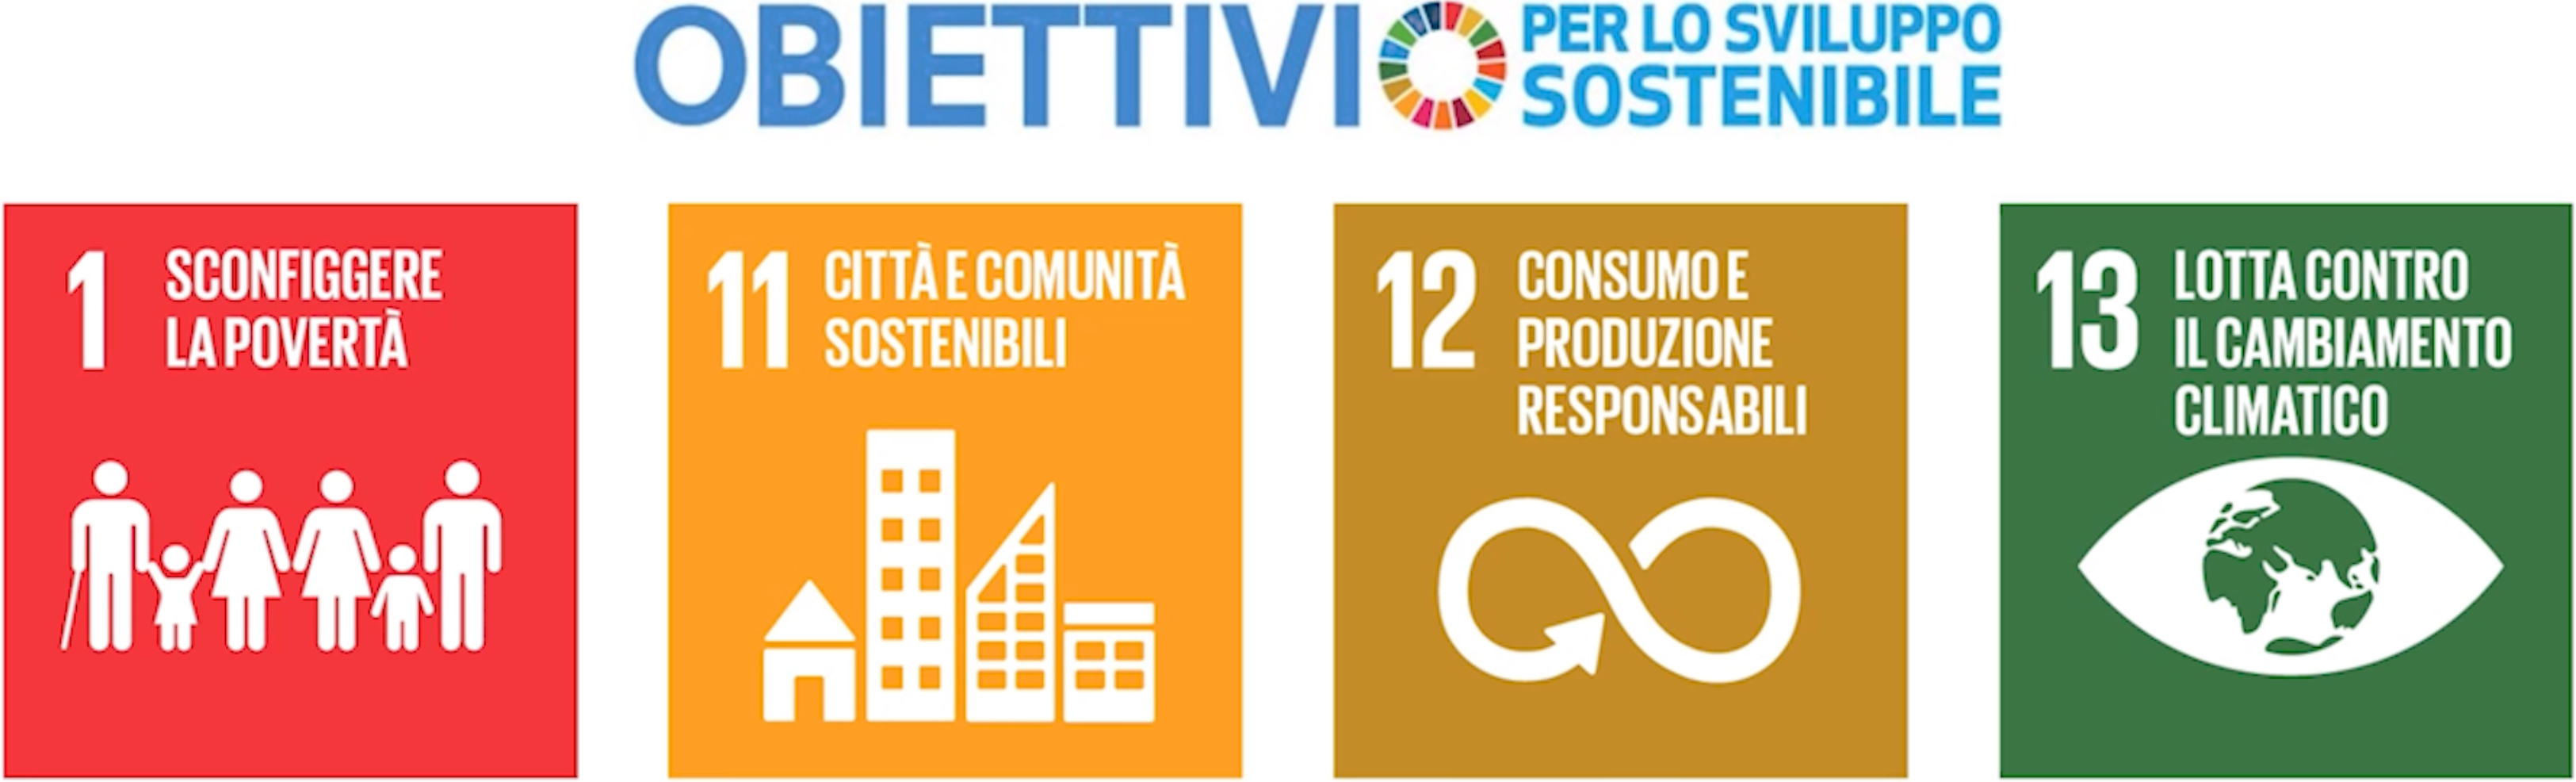
\includegraphics[scale=.075]{images/agenda_2030.png}}
    \hfill
    \caption{Prototipo dell'applicazione mobile}
\end{figure}

Gli utenti potranno ottenere dei Green Coin attraverso le seguenti modalità:
\begin{itemize}
    \item 
    Registrazione sulla piattaforma: verrà fornito un Green Coin alla registrazione (obbligatoria);
    \item Condivisione della piattaforma sui propri canali Social: all’utente che condividerà e pubblicizzerà online l’applicazione verrà dato un Green Coin. Questa modalità si rinnoverà mensilmente, perciò gli utenti potranno ottenere un Green Coin ogni mese semplicemente pubblicizzando la piattaforma che ne guadagnerà in popolarità ed utenti, fidelizzando anche i propri clienti; 
    \item Inserimento di oggetti in offerta nel Marketplace: l’utente potrà inserire oggetti a patto che siano funzionanti e in buone condizioni, otterrà un Green Coin per ogni oggetto inserito nel Marketplace e ceduto ad un altro utente;
    \item Dimostrare di essere in una situazione di difficoltà economica attraverso la dichiarazione dei redditi o l’attestazione ISEE, a tali utenti verranno forniti mensilmente dai 2 ai 5 Green Coin.
\end{itemize}
Abbiamo ideato questa moneta di scambio per risolvere una problematica appartenente a tutti gli attuali centri del riuso fisici: la presenza di utenti che abusano della piattaforma richiedendo una grande mole di oggetti, senza mai contribuire al sistema offrendone altrettanti. 
\medskip

Gli utenti dopo la registrazione potranno accedere alla piattaforma ed usufruire dei servizi che essa offre; una volta collegato l’utente potrà:  
\begin{itemize}
    \item Acquistare un oggetto di cui necessita attraverso la pagina “Acquista”. Nella pagina saranno presenti tutti gli oggetti offerti da utenti membri della piattaforma nella vicinanza dell’utente. Verrà data anche la possibilità di cercare un determinato oggetto all’interno del Marketplace. L’utente interessato ad un oggetto potrà spendere un Green Coin per contattare l’utente offerente e accordarsi per lo scambio dell’oggetto. Nel caso in cui lo scambio non si sia concluso con successo l’utente richiedente otterrà il Green Coin che aveva speso per contattare l’utente offerente. Verrà sempre chiesta conferma ad entrambi gli utenti dell’avvenuto scambio con possibilità anche di rilasciare un feedback;
    \item Offrire un oggetto attraverso la pagina “Offri”. Nella pagina sarà possibile aggiungere un oggetto da offrire nel Marketplace, saranno richieste una breve descrizione e delle foto rappresentative dell’oggetto. Verrà resa pubblica anche la posizione dell’oggetto. Nel caso qualcuno sia interessato all’oggetto verrà contattato e se lo scambio si concluderà con successo l’utente offerente otterrà un Green Coin;
    \item Controllare le proprie transazioni attraverso la pagina “Transazioni”. L’utente potrà visualizzare tutte le sue transazioni, i dettagli relativi ad esse e lo stato attuale: “In Corso”, “Conclusa senza Successo” e “Conclusa con Successo”;
    \item Controllare il proprio bilancio attraverso la pagina “Bilancio”. L’utente potrà visualizzare il bilancio del suo profilo, quindi i movimenti dei Green Coin in entrata ed uscita;
    \item Visualizzare e modificare il proprio profilo attraverso la pagina “Profilo”. L’utente potrà visualizzare il proprio profilo e modificare i dati relativi ad esso. Per gli scambi è molto importante la posizione dell’utente;
\end{itemize}